% NOTES:
%   - Core message: realistic sequences expose session and refinement effects,
%     other evaluation methods miss them or point to the wrong conclusion
%   - Session chart is drawn from Table 2 of the paper (mean over all 9 cache configurations)

\begin{frame}{Results: All Caches Outperform No Caching}
    \centering
    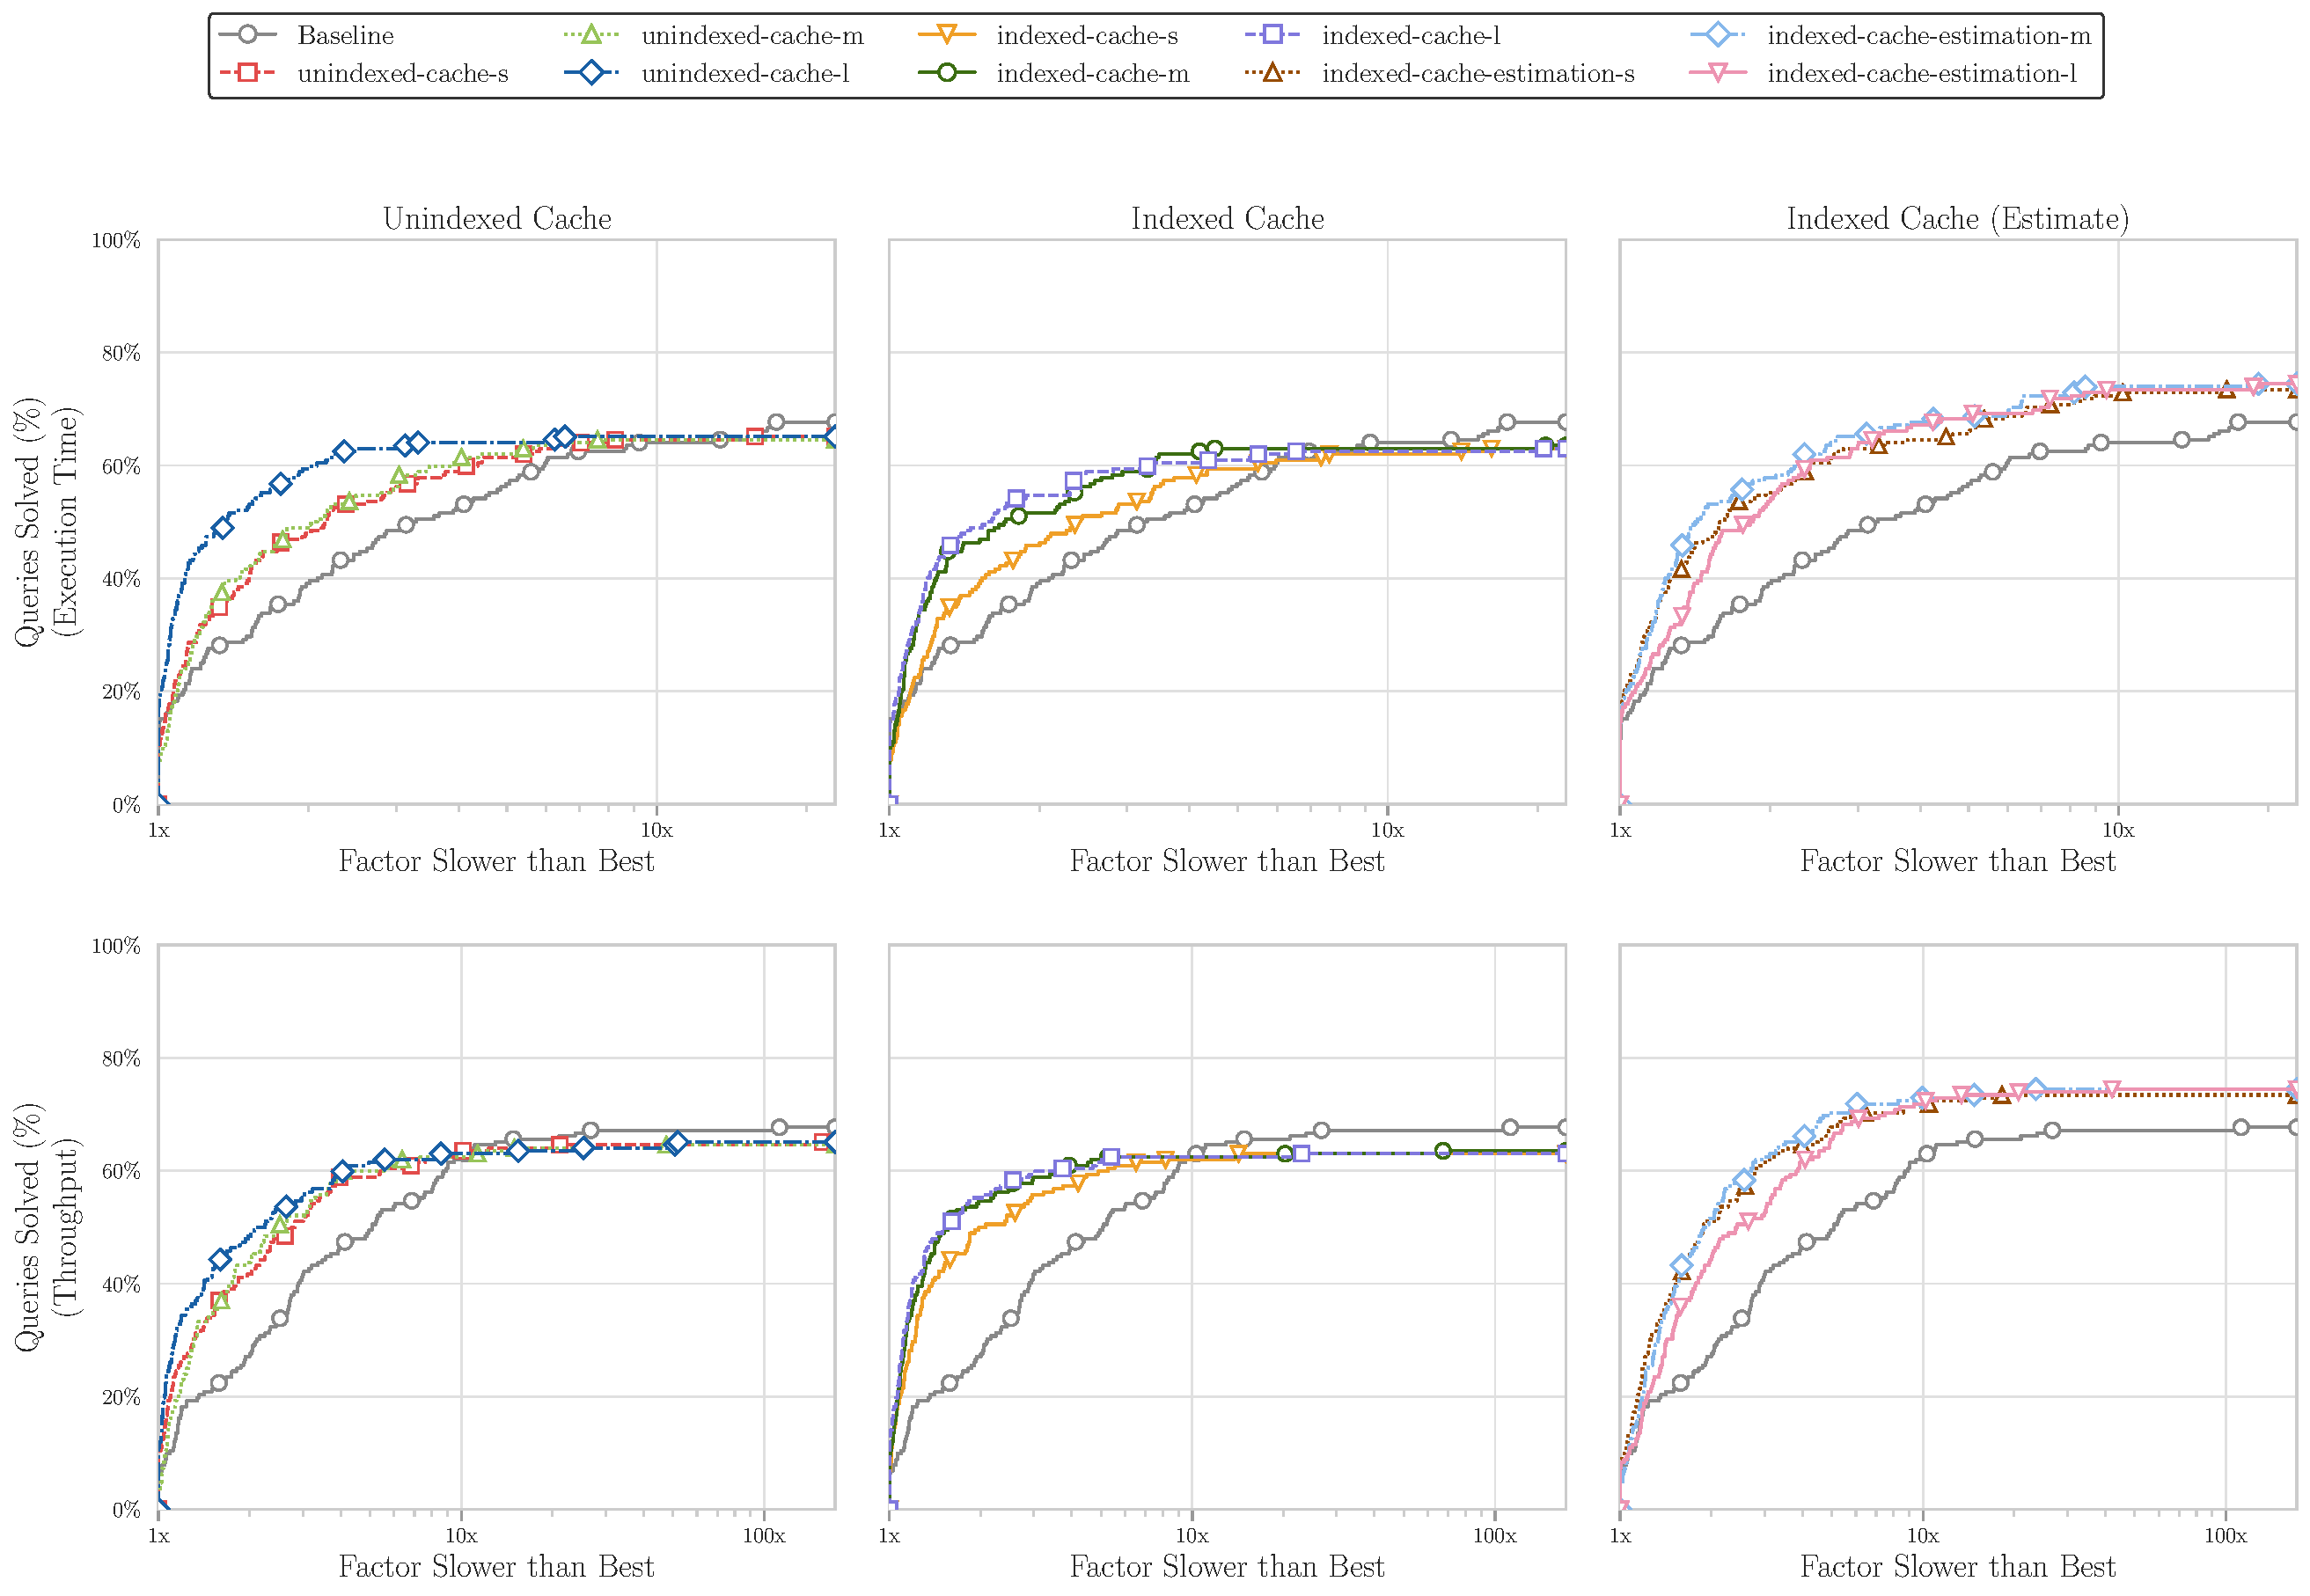
\includegraphics[width=.88\linewidth,trim=0 393 0 0,clip]{images/performance_profile.pdf}

    \footnotesize
    Performance profile \parencite{dolan2002benchmarking}: higher and further left is better
    \normalsize

    \vspace{0.5em}
    Cardinality estimation performs best and solves the most queries
\end{frame}

\begin{frame}{Results: Session Switching Costs Cache Hits}
    \begin{columns}[T]
        \begin{column}{0.55\textwidth}
            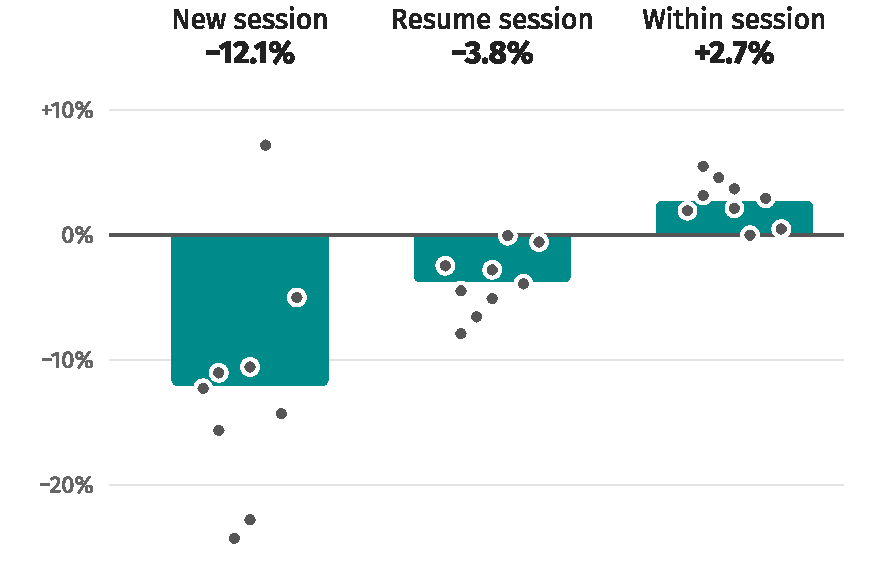
\includegraphics[width=\linewidth]{images/session-hit-rates.pdf}
        \end{column}

        \begin{column}{0.45\textwidth}
            \begin{itemize}
                \item Hit rate compared to the average of the same template
                \item New sessions: $-12\%$
                \item Staying in a session: $+3\%$
                \item[$\Rightarrow$] Cache sizing and eviction depend on session behavior
            \end{itemize}
        \end{column}
    \end{columns}
\end{frame}

\begin{frame}{Results: Refinement Reuses Prior Data}
    \centering
    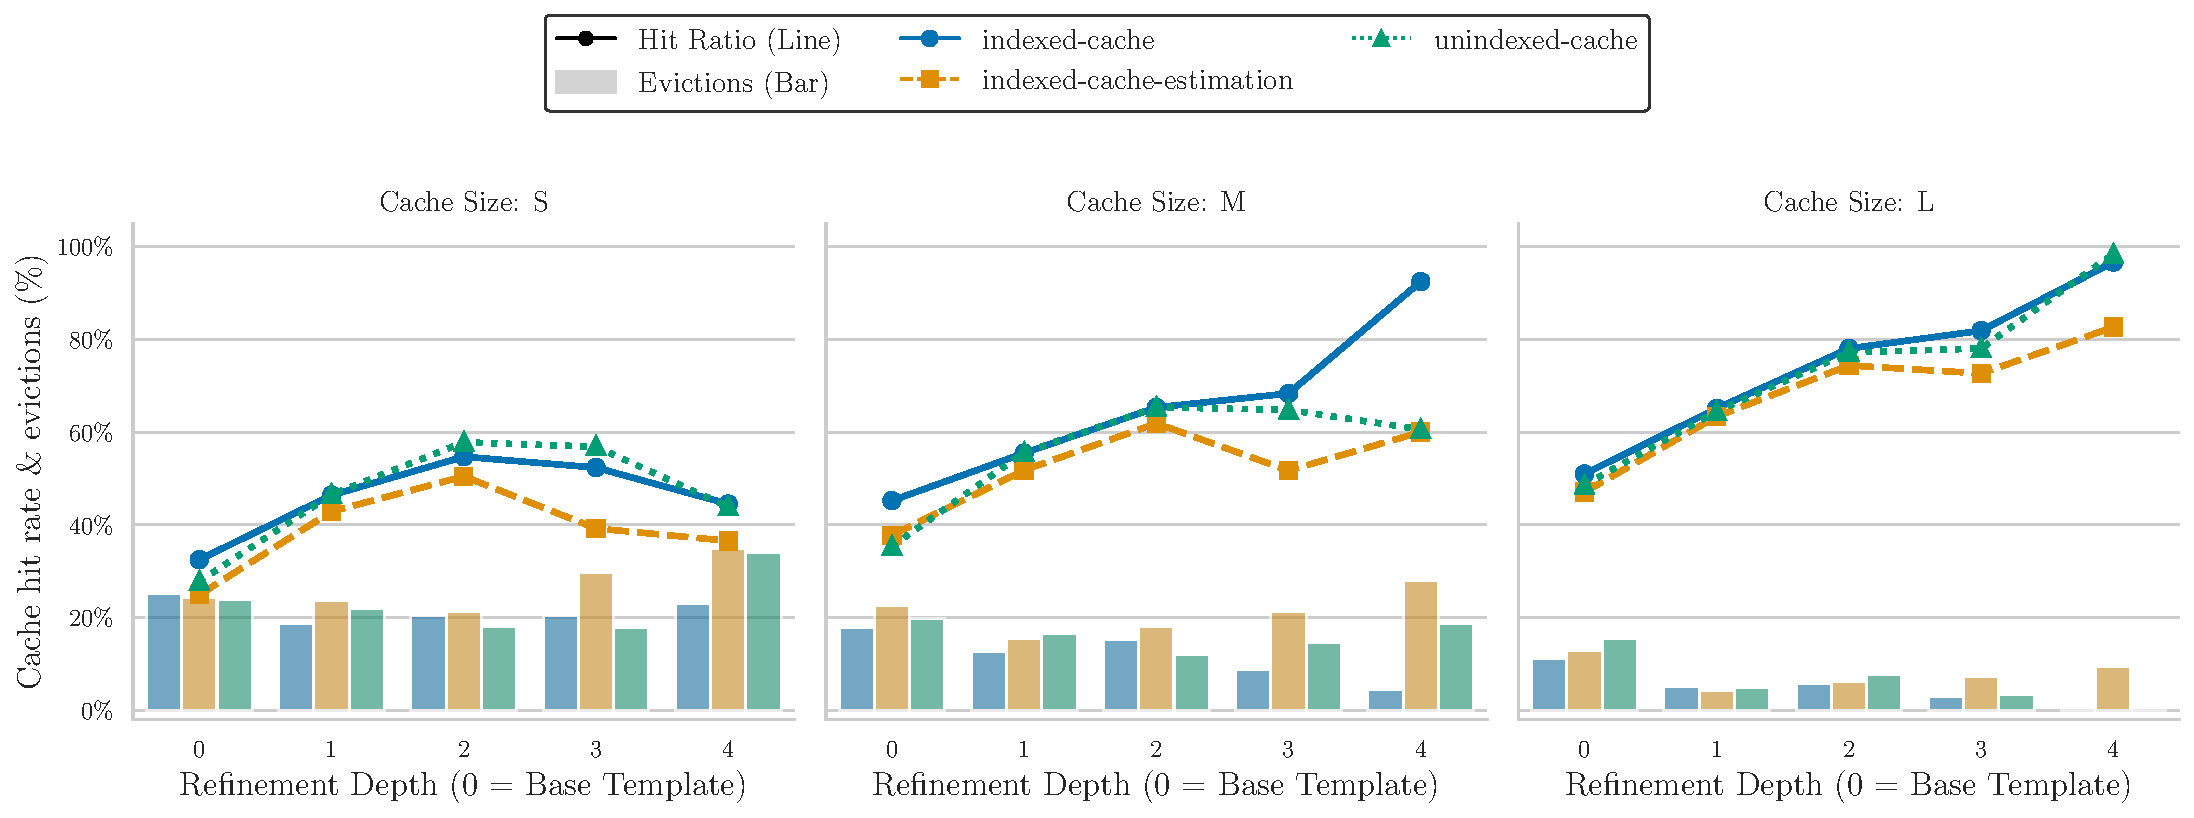
\includegraphics[width=\linewidth]{images/combined_cache_efficiency.pdf}

    \vspace{0.5em}
    Hit rates rise with each refinement step, until small caches start thrashing
\end{frame}

\begin{frame}{Results: Refinement Translates into Speedups}
    \centering
    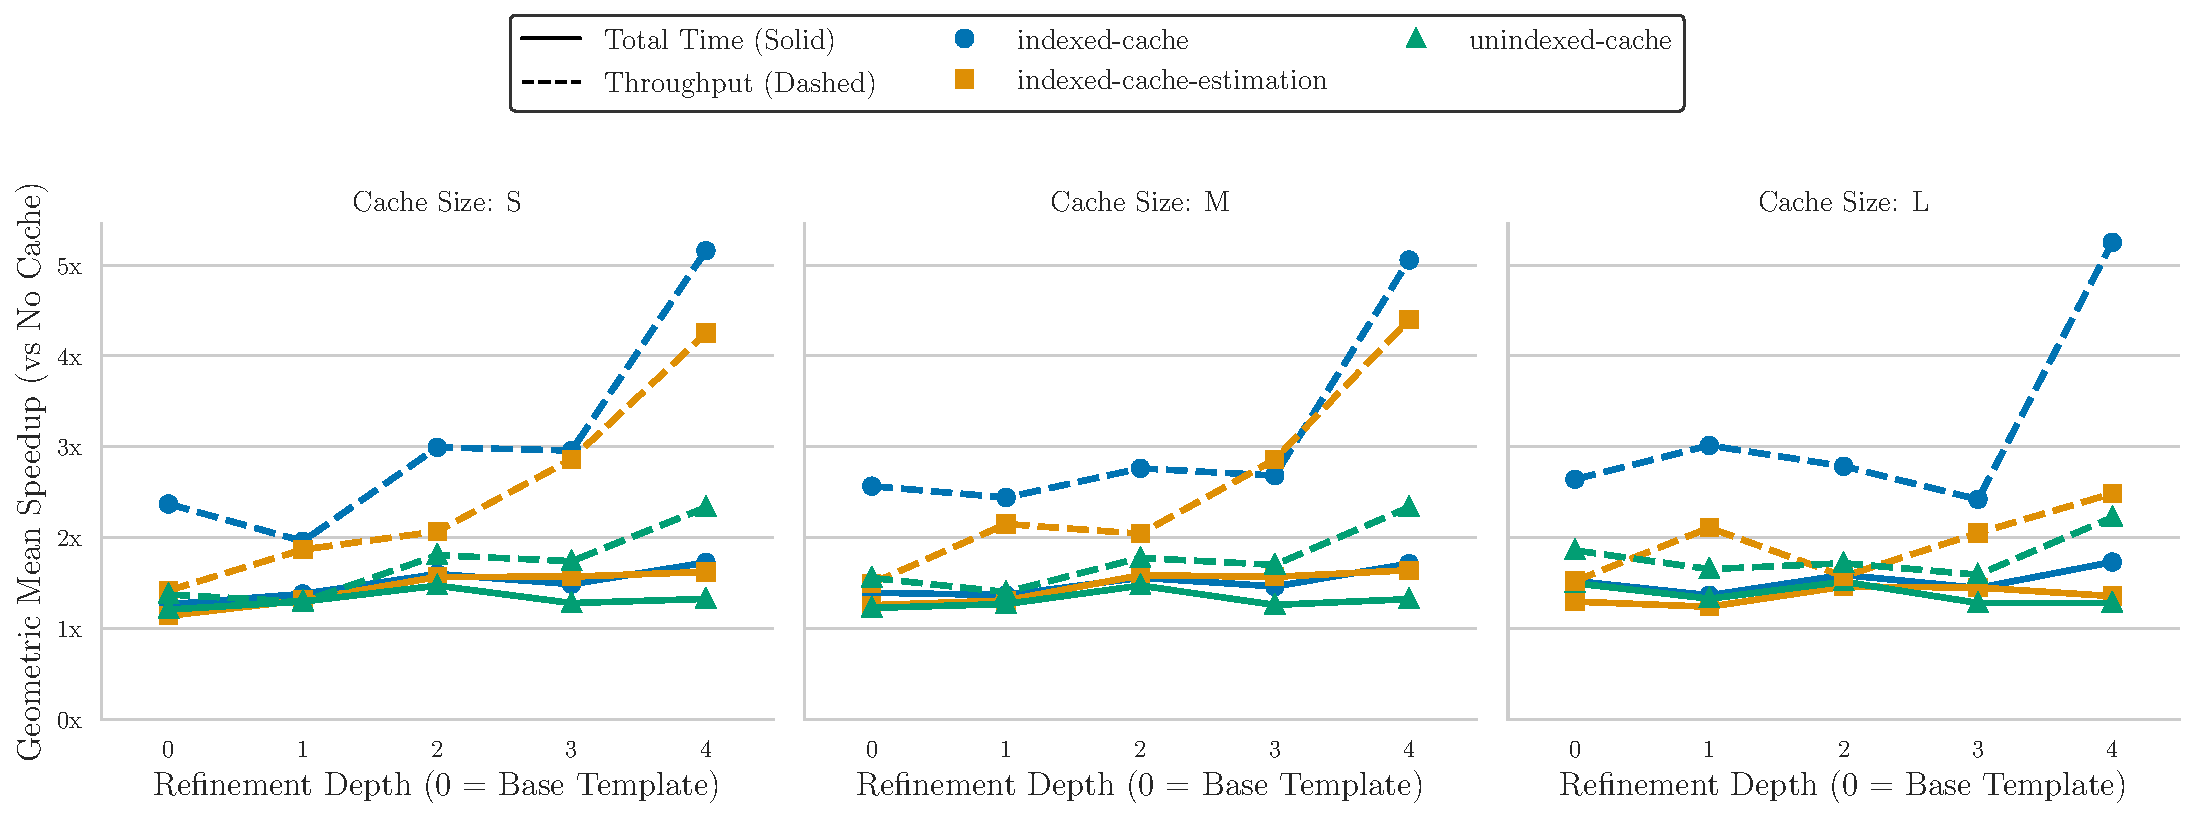
\includegraphics[width=\linewidth]{images/temporal_throughput_line.pdf}

    \vspace{0.5em}
    Up to $\sim$5$\times$ throughput at refinement depth 4 with the indexed cache
\end{frame}

\begin{frame}{Comparison: Random Sequences Mislead}
    % Paper legends cropped off; random panel scaled so both plot areas have the same height
    \begin{columns}[T]
        \begin{column}{0.5\textwidth}
            \centering
            \textbf{Random sequences}

            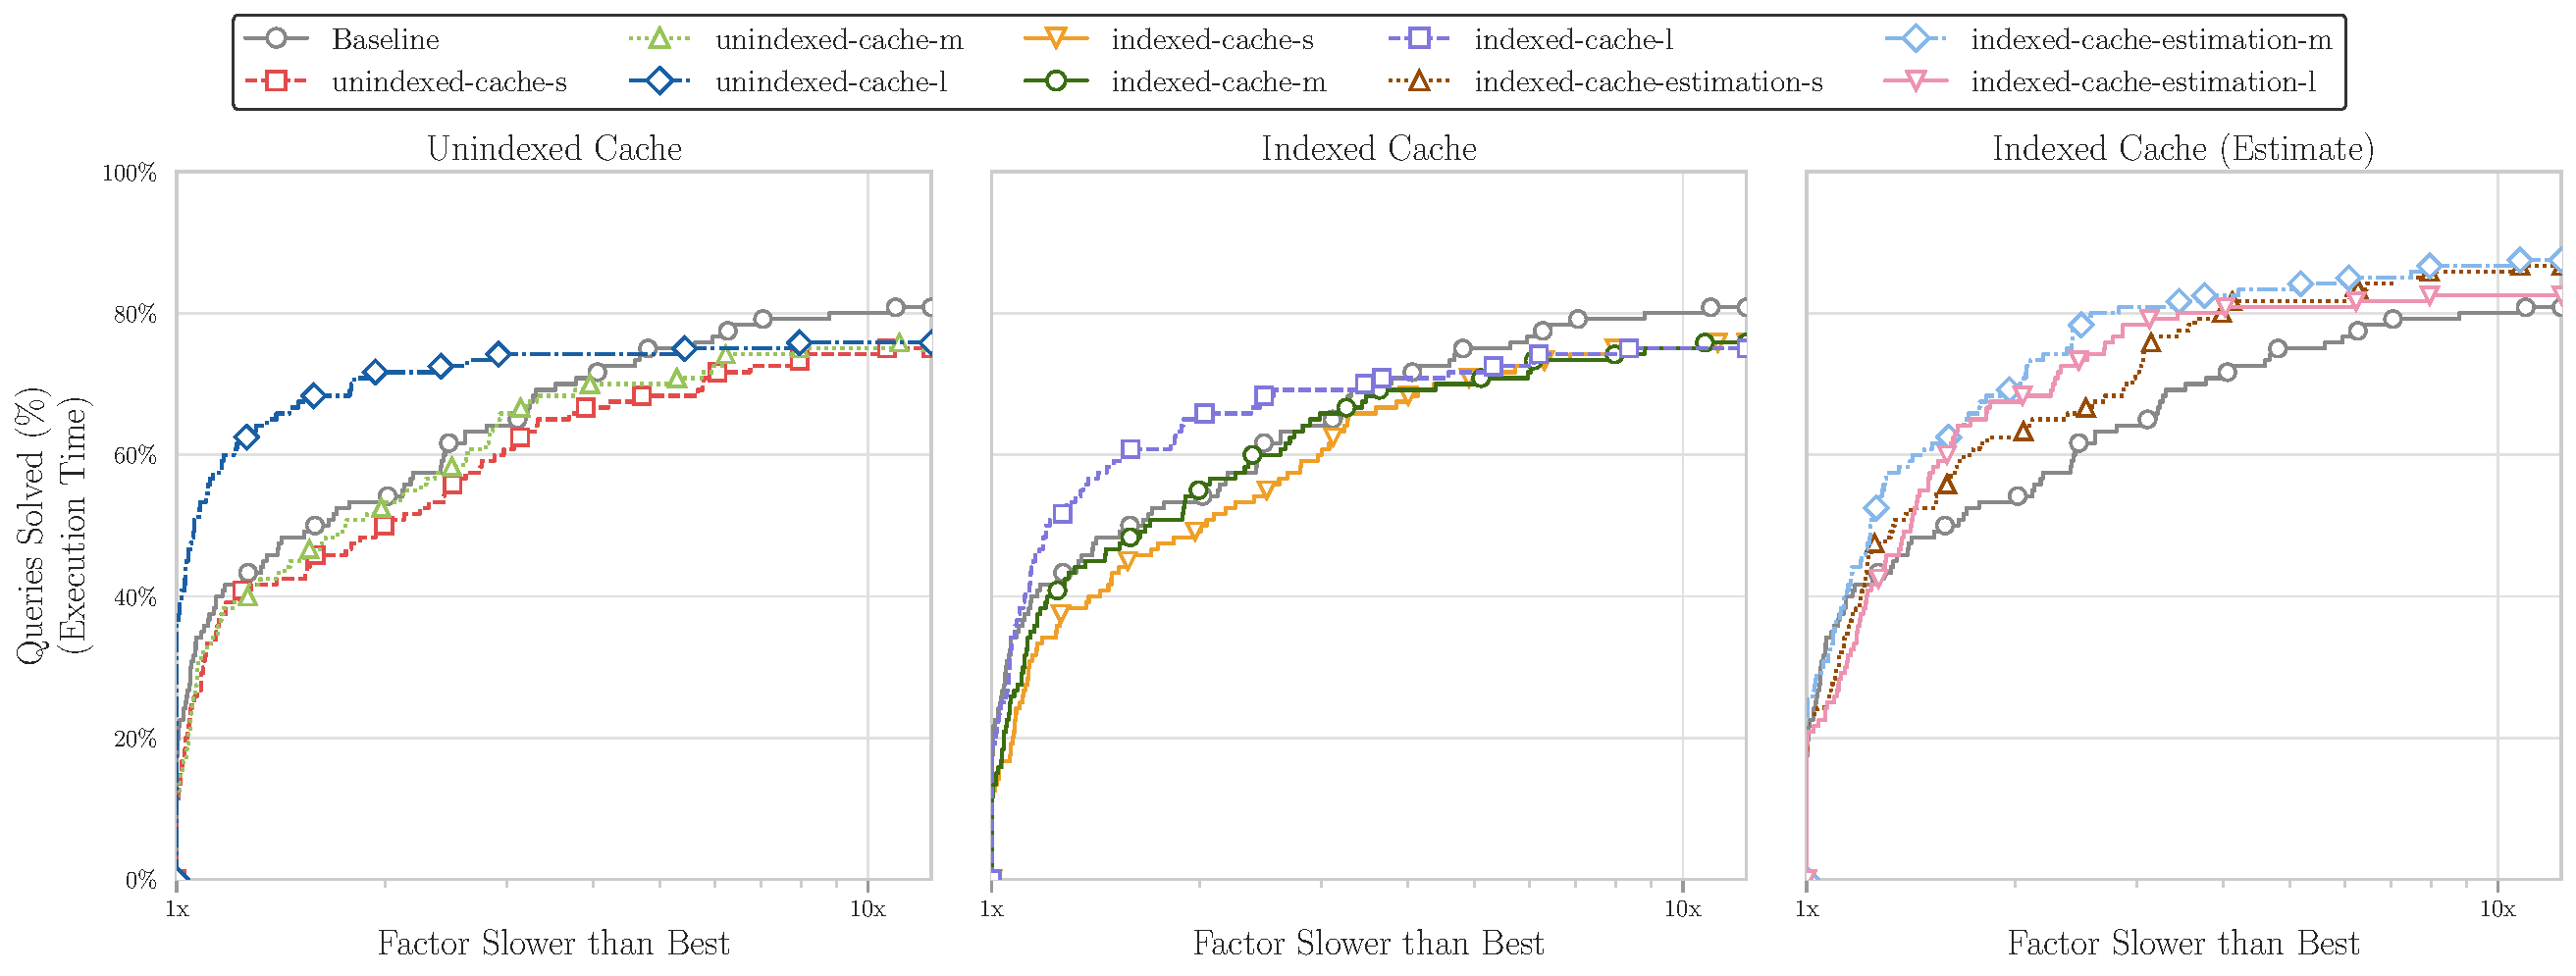
\includegraphics[width=.72\linewidth,trim=0 0 803 80,clip]{images/performance_profile_random_sequences.pdf}
        \end{column}

        \begin{column}{0.5\textwidth}
            \centering
            \textbf{SolidSessionBench}

            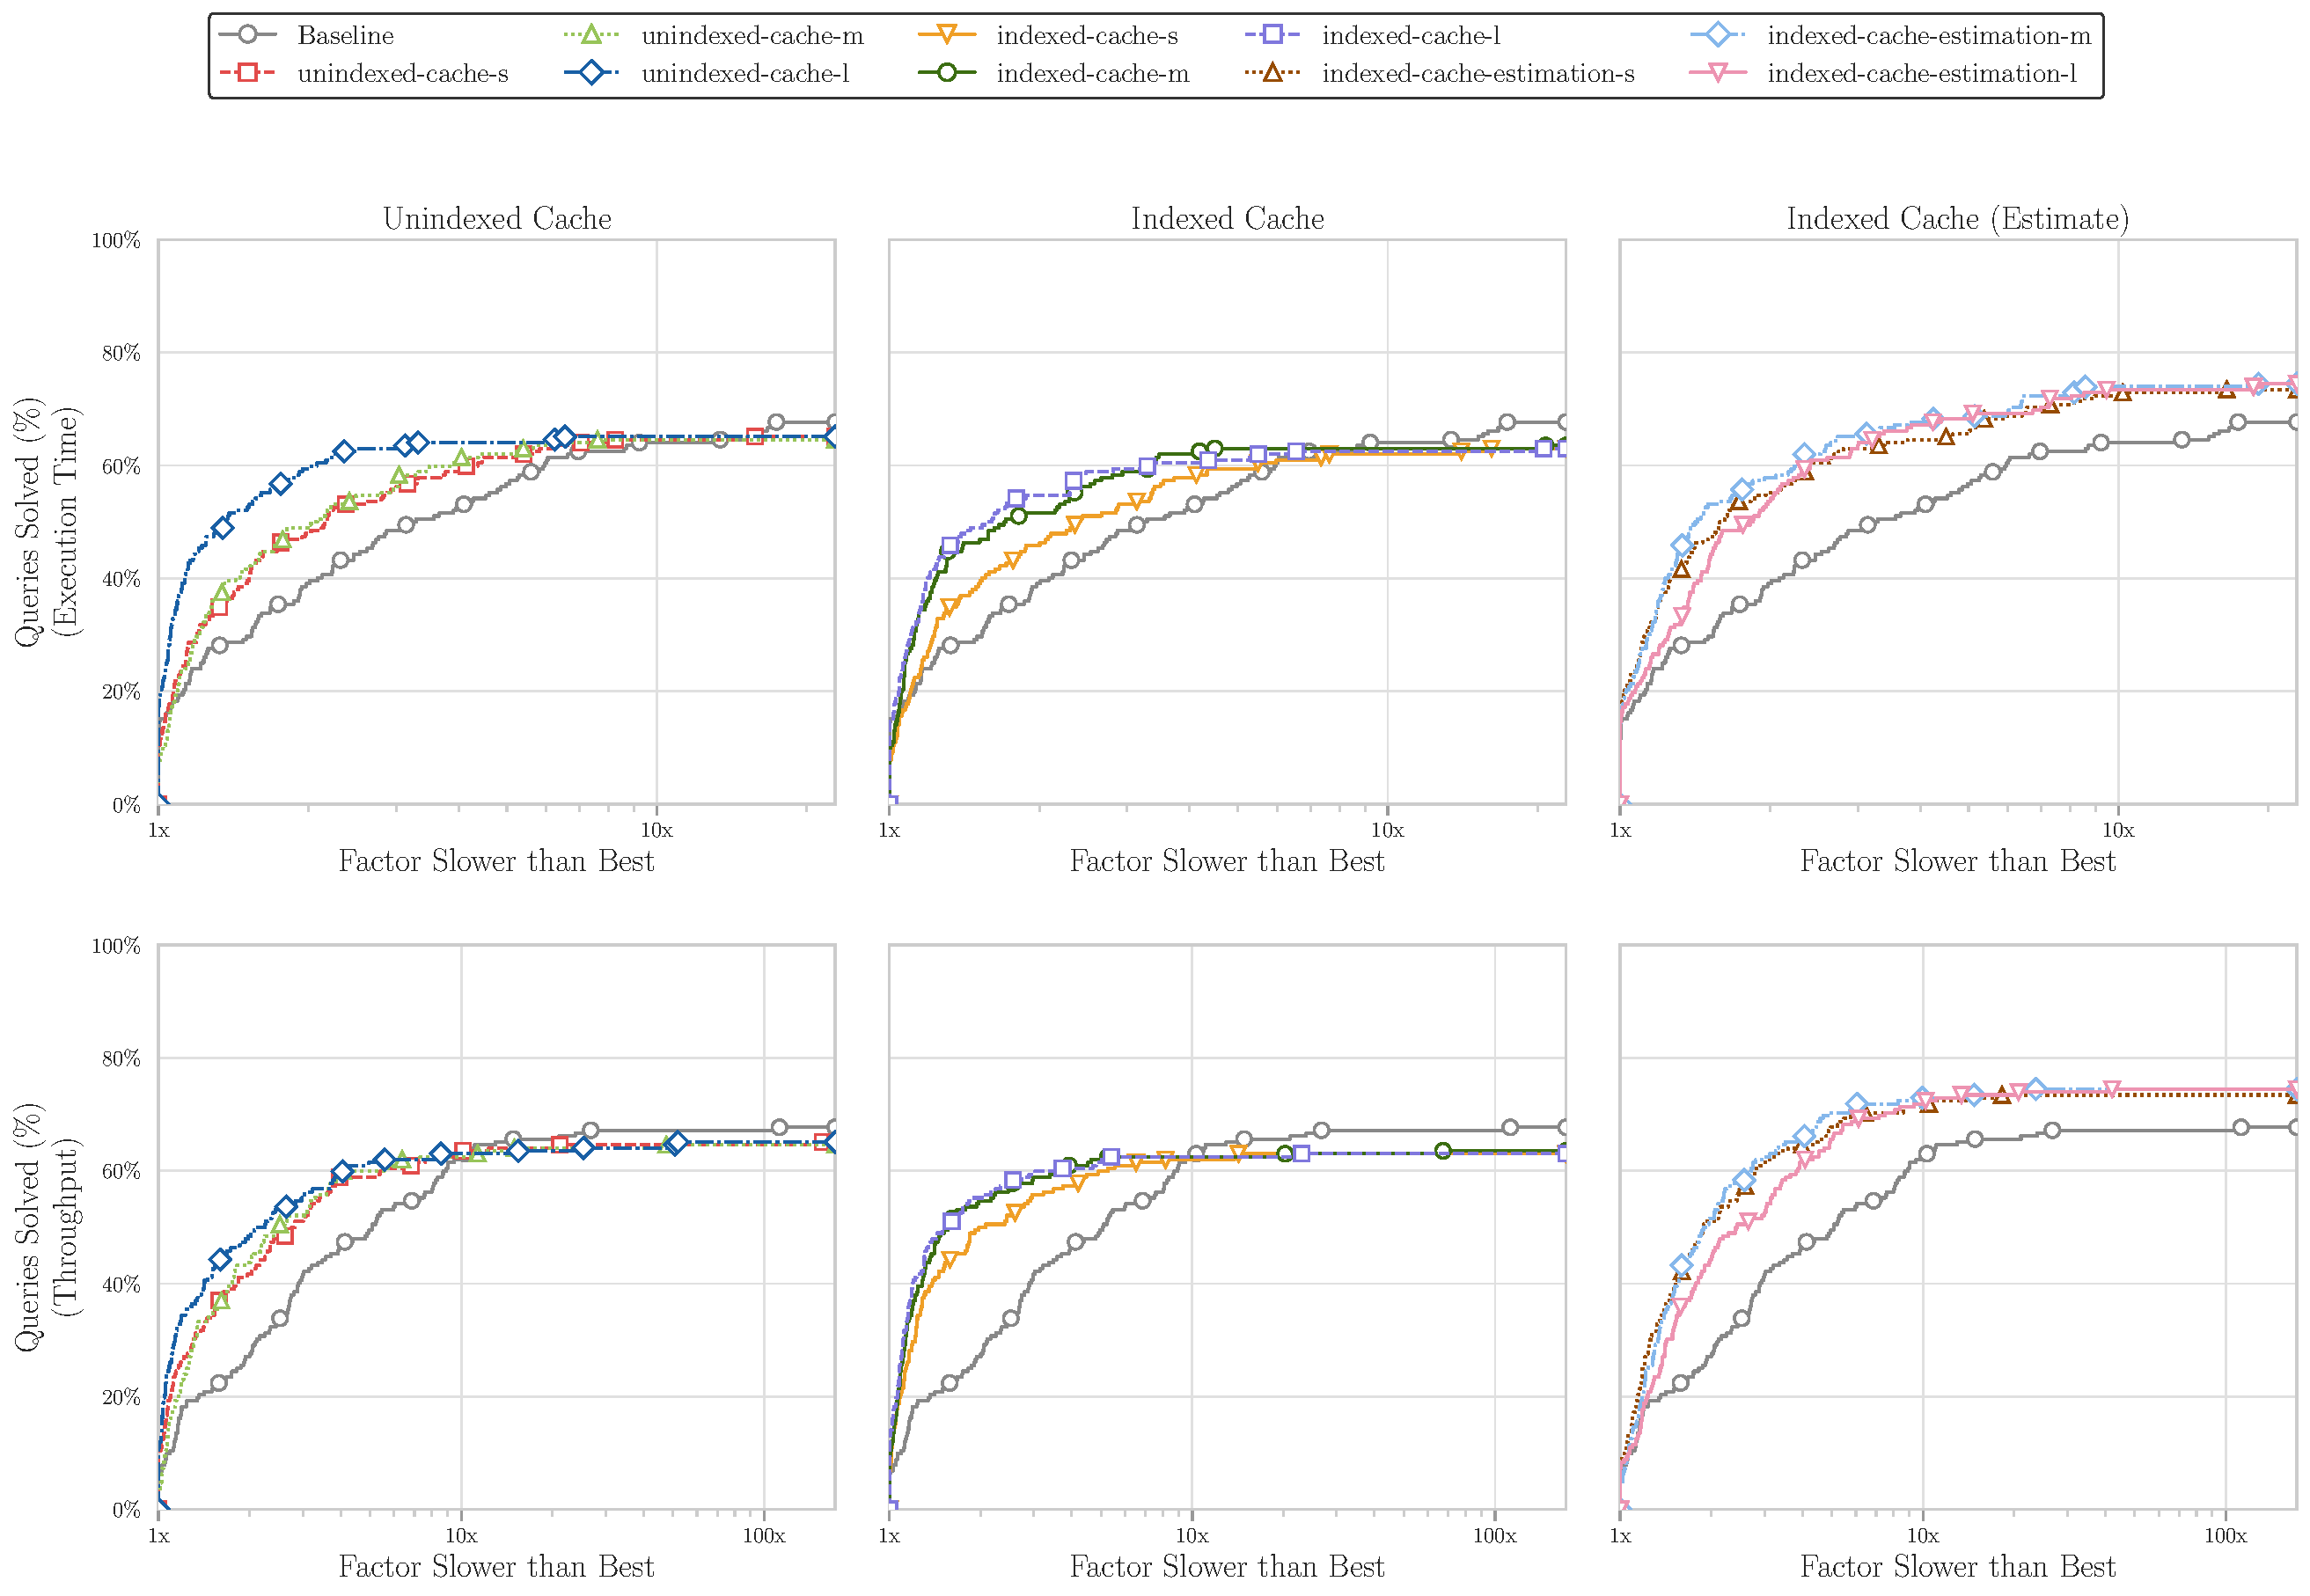
\includegraphics[width=.81\linewidth,trim=0 390 803 125,clip]{images/performance_profile.pdf}
        \end{column}
    \end{columns}

    \vspace{0.3em}
    \centering
    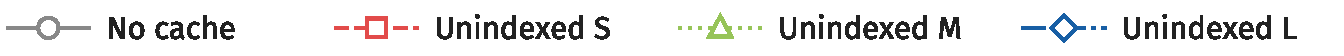
\includegraphics[width=.7\linewidth]{images/legend-unindexed.pdf}

    \vspace{0.5em}
    Random: only large caches help \quad vs.\ \quad SolidSessionBench: small caches help too
\end{frame}

\begin{frame}{Comparison: Micro Benchmarks Give Mixed Signals}
    \begin{columns}[T]
        \begin{column}{0.6\textwidth}
            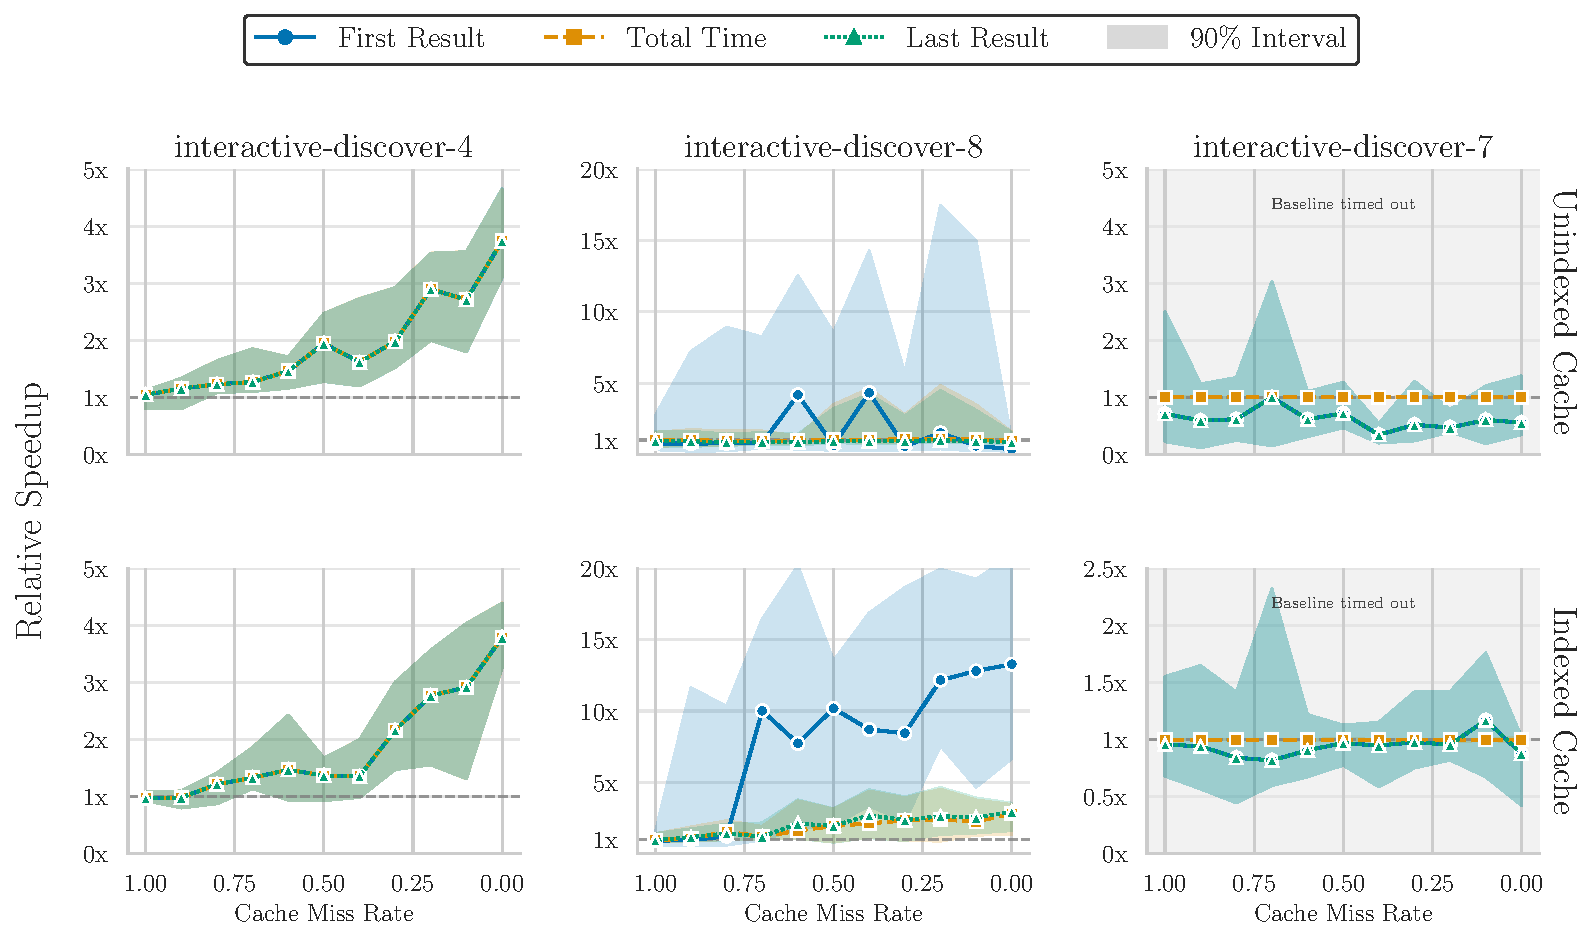
\includegraphics[width=\linewidth]{images/synth_hit_rate_reduced.pdf}
        \end{column}

        \begin{column}{0.4\textwidth}
            \begin{itemize}
                \item Each template run twice with simulated cache miss rates
                \item 8 of 12 templates speed up with hit rate
                \item Long-running queries: no speedup, or even slowdowns
                \item[$\Rightarrow$] Isolated queries do not show behavior in realistic sequences
            \end{itemize}
        \end{column}
    \end{columns}
\end{frame}

\begin{frame}{Key Takeaways}
    \begin{itemize}\setlength\itemsep{1.5em}
        \item Realistic sequences reveal how sessions and refinement drive client-side performance
        \item Random sequences and micro benchmarks miss these effects, or lead to the wrong conclusions
        \item[$\Rightarrow$] SolidSessionBench: a reproducible basis for evaluating client-side optimizations
    \end{itemize}
\end{frame}
